\documentclass[12pt,a4paper]{article}

\usepackage{amsmath}
\usepackage{amssymb}
\pagestyle{empty}
\usepackage[margin=1cm]{geometry}
\usepackage{hyperref}
\usepackage[utf8]{inputenc}
\usepackage[IL2]{fontenc}
\usepackage[czech]{babel}
\usepackage{graphicx}

\DeclareMathOperator{\tg}{tg}
\def\ee{\mathrm{e}}
\def\dd{\,\mathrm{d}}

\def\tisk{%
\newbox\shipouthackbox
\pdfpagewidth=2\pdfpagewidth
\let\oldshipout=\shipout
\def\shipout{\afterassignment\zdvojtmp \setbox\shipouthackbox=}%
\def\zdvojtmp{\aftergroup\zdvoj}%
\def\zdvoj{%
 	\oldshipout\vbox{\hbox{%
       	\copy\shipouthackbox
        \hskip\dimexpr .5\pdfpagewidth-\wd\shipouthackbox\relax
        \box\shipouthackbox
    }}%
}}%


\begin{document}

%\tisk

\section*{Plochy a obsahy}

%\emph{Výsledky jsou na druhé straně.}

\def\vysl#1{\hfill#1\par}
\def\cb#1{$\vcenter{\hbox{#1}}$\quad\ignorespaces}

\begin{enumerate}
	%\everymath{\displaystyle}
	\parskip\medskipamount
	\item Spočtěte obsah útvaru ohraničeného osou $x$ a funkcí $y = x^2 - 4$. %\cb{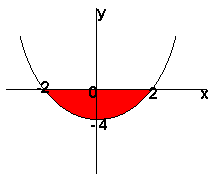
\includegraphics[scale=.4]{parabola_pod.png}}
	\item Spočtěte obsah útvaru ohraničeného přímkami $x=-2$, $x = 2$, osou $x$ a funkcí $y = x^3$. %\cb{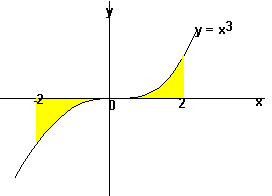
\includegraphics[scale=.4]{cube.png}}
	\item Spočtěte obsah útvaru na obrázku (ta funkce je $y = x^2$). %\cb{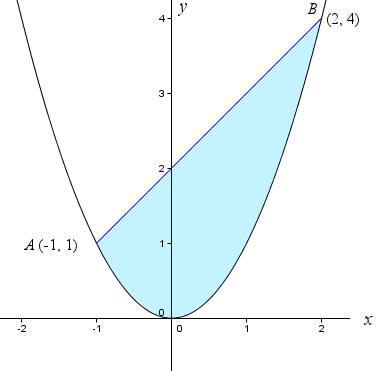
\includegraphics[scale=.37]{usek_paraboly.png}}
	\item (Pro gurmány) Spočtěte obsah srdíčka, jehož hranice je tvořena křivkou o rovnici $|x| + \bigl(y-\sqrt{|x|}\bigr)^2 = 1$. %\cb{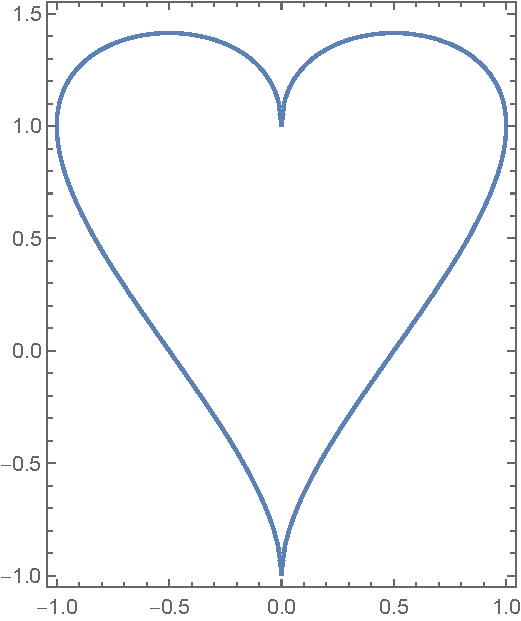
\includegraphics[scale=.4]{srdce.pdf}}
	\item Vymyslete úlohu na obsah útvaru, kterou umíte (snadno a rychle) vypočítat, a zadejte ji dvěma jiným skupinám.
	\item Vyřešte úlohy, které jste dostali od jiných skupin, a ohodnoťte je na stupnici 0--5 hvězdiček.
	\item Spočtěte objem rotačního kužele o výšce $v$ a poloměru podstavy $r$.
	\item Spočtěte objem koule o poloměru $r$ (jednodušší varianta: $r = 1$).
	\item Spočtěte objem kulového vrchlíku o výšce $h$ useklého z koule o poloměru $r$.
	\item Chladící věže (např. jaderných elektráren) mají tvar rotačních hyperboloidů. Spočtěte, jaký objem bude mít chladící věžička, která vznikne rotací hyperboly $x^2 - y^2 = 1$ okolo osy $y$, přičemž její spodek bude v $y = -2$ a vršek v $y = 1$.
	\item Jaký bude objem doprava nekonečné zužující se roury, která začíná v $x = 1$ a vznikne rotací grafu $y = \frac1x$ okolo osy $x$?
	\item Spočtěte objem kapky, která vznikne rotací grafu funkce $y = \sqrt{x} - x$ okolo osy $x$, přičemž $x$ jde od $0$ do $1$. Pokud nevíte coby, tak si ještě spočtěte, jak je ta kapka široká v nejširším místě.
	%\item 
\end{enumerate}


\subsection*{Obrázky k úlohám}

\begin{flushleft}
\bfseries
1. \cb{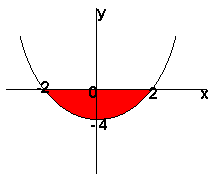
\includegraphics[scale=.4]{parabola_pod.png}}
2. \cb{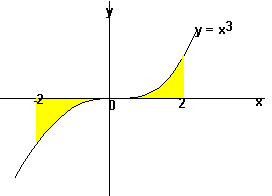
\includegraphics[scale=.4]{cube.png}}
3. \cb{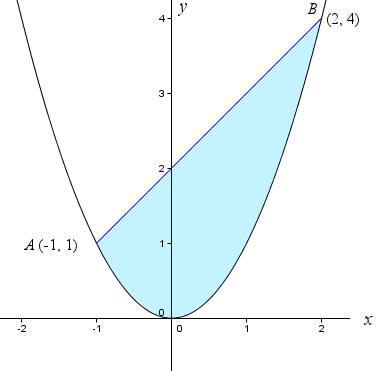
\includegraphics[scale=.37]{usek_paraboly.png}}
4. \cb{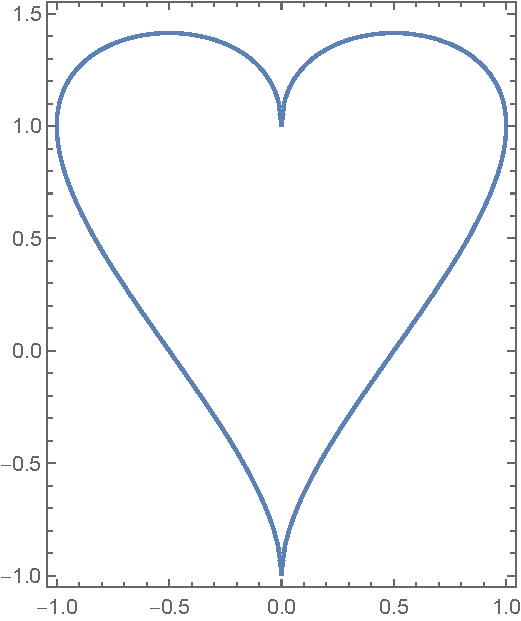
\includegraphics[scale=.4]{srdce.pdf}}
10. \cb{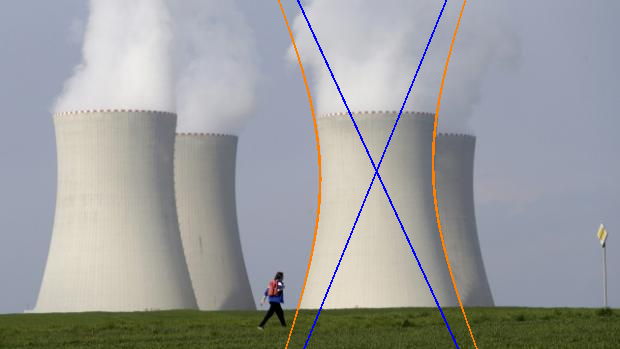
\includegraphics[scale=.4]{temelin.png}}
12. \cb{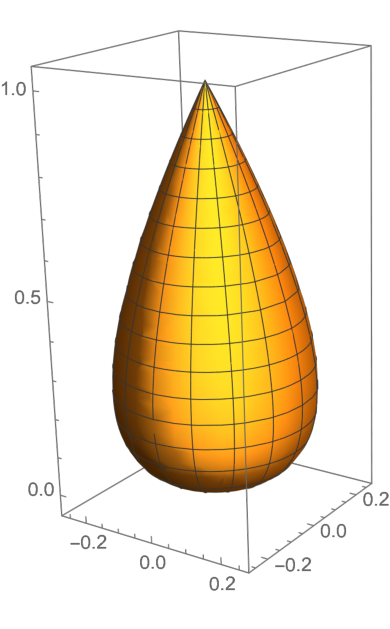
\includegraphics[scale=.6]{kapka.pdf}}
\end{flushleft}


\end{document}